% Technische Universität Dresden
% Fakultät Informatik
% Institut für Software- und Multimediatechnik
% Seniorprofessur für Multimediatechnik
%
% Example document demonstrating the usage of mmthesis.sty
% 2012-10-26 Andreas Rümpel
% 
% ### build hints (% = filename of tex file) ###
% pdflatex: pdflatex %.tex
% biber: biber % (biber is a modern backend for bibtex, http://biblatex-biber.sourceforge.net)
% glossaries and acronyms: makeglossaries %
%
% Das LATEX2e-Sündenregister: ftp://ftp.dante.de/tex-archive/info/l2tabu/german/l2tabu.pdf
% KOMAScript-Guide: ftp://ftp.dante.de/tex-archive/macros/latex/contrib/koma-script/scrguide.pdf
% Einige typographische Grundregeln und ihre Umsetzung in LaTeX: http://www2.informatik.hu-berlin.de/sv/lehre/typographie.pdf

\documentclass[
	headsepline,
	footsepline,
	fontsize=12pt,
	%draft, % use this for finding overfull boxes
	%parskip, % use this for alternative paragraph formatting
	bibliography=totoc
]{scrbook}


\usepackage[utf8]{inputenc}
\usepackage{mmthesis}
\addbibresource{library.bib} % put name of bib file here with extension

%### switches
%\printoutput % make link colors black, leave deactivated for screen output

%### define metadata
\mmtype{Diplomarbeit} %Diplomarbeit|Großer Beleg|Bachelorarbeit|Masterarbeit|Seminararbeit
\mmtitle{Semantik-gestütztes Hilfesystem für ein komposites Informationsvisualisierungssystem}
\mmtshorttitle{Hilfesystem für komposite InfoVis}
\mmtauthor{Nikolaus Piccolotto}
\mmtsubmissionmonth{November 2013}
\mmtsubmissiondate{30. November 2013}
\mmtsupervisor{Dipl.-Medieninf. Martin Voigt}
%\mmtsupervisorii{Dipl.-Medieninf. Foo Bar} % Co-supervisor, optional

\mmthypersetup % has to be called after setting metadata

%### acronyms
\newacronym{PDF}{PDF}{Portable Document Format}
\newacronym{RCP}{RCP}{Rich Client Platform}
\newacronym{RIA}{RIA}{Rich Internet Application}
\newacronym{RELAXNG}{RELAX NG}{Regular Language Description for XML New Generation}
\newacronym{SGML}{SGML}{Standard Generalized Markup Language}
\newacronym{SWT}{SWT}{Standard Widget Toolkit}
\newacronym{WDC}{W3C}{World Wide Web Consortium}
\newacronym{WPF}{WPF}{Windows Presentation Foundation}
\newacronym{XPath}{XPath}{XML Path Language}
\newacronym{XHTML}{XHTML}{Extensible Hypertext Markup Language}
\newacronym{XML}{XML}{Extensible Markup Language}
% my acronyms
\newacronym{InfoVis}{InfoVis}{Informationsvisualisierung}


\begin{document}
\frontmatter
\pagenumbering{Roman}
\mmtfrontmatter

\listoffigures
\listoftables
\printglossary[type=\acronymtype,style=long,title=Abkürzungsverzeichnis,toctitle=Abkürzungsverzeichnis]
%\printglossary %Glossar

\mainmatter

\chapter{Einleitung}
\label{chapter:einleitung}

% Hier kommt eine kurze Einführung von semantischen Daten, nehme ich an

\section{Motivation}
\label{section:motivation}

% Hier wird generell eingeleitet, also vermutlich die Problematik zwischen semantischen Datensätzen und Endusern

\section{Problemstellung und Zielsetzung}
\label{section:problemstellung}

% Hier wird quasi der Vizboard Workflow umrissen
% und erklärt, wo das eigentliche Problem liegt, nämlich im Information Overload beim letzten Schritt

\begin{figure}[htbp]
	\centering
	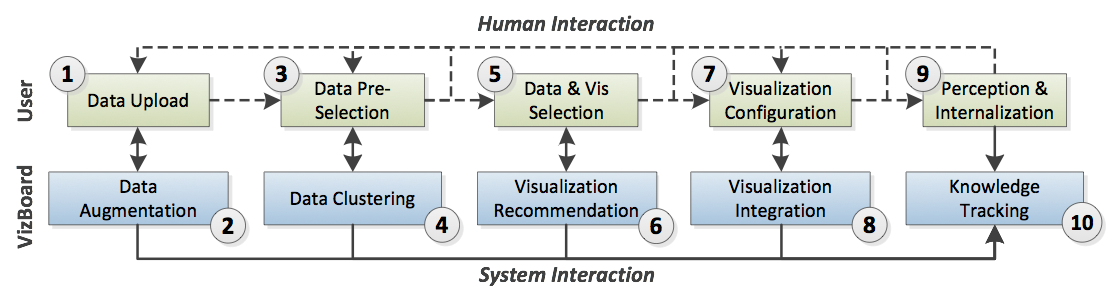
\includegraphics[width=0.75\textwidth]{images/vizboard_workflow.png}
	\caption{VizBoard Workflow}
	\label{figure:vizboard_workflow}
\end{figure}

\section{Aufbau der Arbeit}
\label{section:aufbau}

% Aufbau der Arbeit erklären, kommt zum Schluss

\chapter{Stand der Forschung und Technik}
\label{chapter:standderforschung}

\section{Grundlagen}
\label{section:grundlagen}

\section{Szenario}
\label{section:szenario}

% kurze einleitung noch mal

Wie in Kapitel~\ref{chapter:einleitung} erläutert, ist das komposite InfoVis-System Teil der Anwendung VizBoard. Sie leitet den Benutzer in mehreren Schritten von der Auswahl eines Datensatzes zur finalen, kompositen Informationsvisualisierung. Im vorletzten Schritt wählt dieser mit Hilfe eines Facettenbrowsers geeignete Visualisierungskomponenten aus, welche danach angezeigt werden. Um die Problemstellung noch einmal zu verdeutlichen, wird im folgenden ein mögliches Szenario beschrieben.

% einführung der problemstellung
Alice möchte für ihr Biologiestudium mehr über die geografische Verteilung verschiedener Genvarationen herausfinden. Dazu sucht sie im Internet nach einem Datensatz, welchen sie auch findet. Leider ist er in einem für Alice unbekannten Format abgespeichert, nämlich OWL. Außerdem ist er ca. 30\,MB groß, das ist zu viel um es manuell zu verarbeiten. Davon abgesehen sind geografische Breite und Länge als Zahlenkombination keine anschauliche Repräsentation von Orten. Alice hört von einem Freund, dass VizBoard gut geeignet ist um semantische Datensätze anzusehen und probiert es aus.

% Der Benutzer ist laut unserem Rollenmodell weder Developer noch Visualisierungsexperte, d.h. er hat erstmal Schwierigkeiten zu erfassen, was hier überhaupt abgeht

Nachdem Alice ihren Datensatz auch bei VizBoard gefunden und die gewünschten Visualisierungskomponenten (eine Karte, ein Balkendiagramm, eine Tabelle und eine Treemap) ausgewählt hat, werden diese ihr angezeigt. Alice benutzt VizBoard zum ersten Mal und macht außer Facebook und YouTube auch sonst nicht viel im Internet, das heißt sie ist zunächst von den vier unterschiedlichen Fenstern etwas überfordert.
% lösungsansätze!

% Was sind das für Fenster? Welche Komponente ist welche? Welche macht was? Wie kann ich sie bedienen? HUUUPS da ändert sich ja was obwohl ich dort nix gemacht hab! Wie hängen die zusammen? Was sind das für Daten, die dargestellt werden? Was heißt GDP? Wie wird das berechnet? Was soll die Spitze bei 1990? Woher kommt die? Diese eine Komponente scheint kaputt zu sein, wo kann ich mich beschweren?

\chapter{Konzept}

\section{Anforderungsanalyse}

%### end of appendix
%#####################################################
\printbibliography[title=Literaturverzeichnis]

%\printindex

\end{document}